\begin{figure}[t]
    \centering
    % \includegraphics[width=0.45\textwidth,trim={0 0 0 170mm},clip]{figures/skorch_lr_recalls_at_various_target_precisions_test.pdf}
    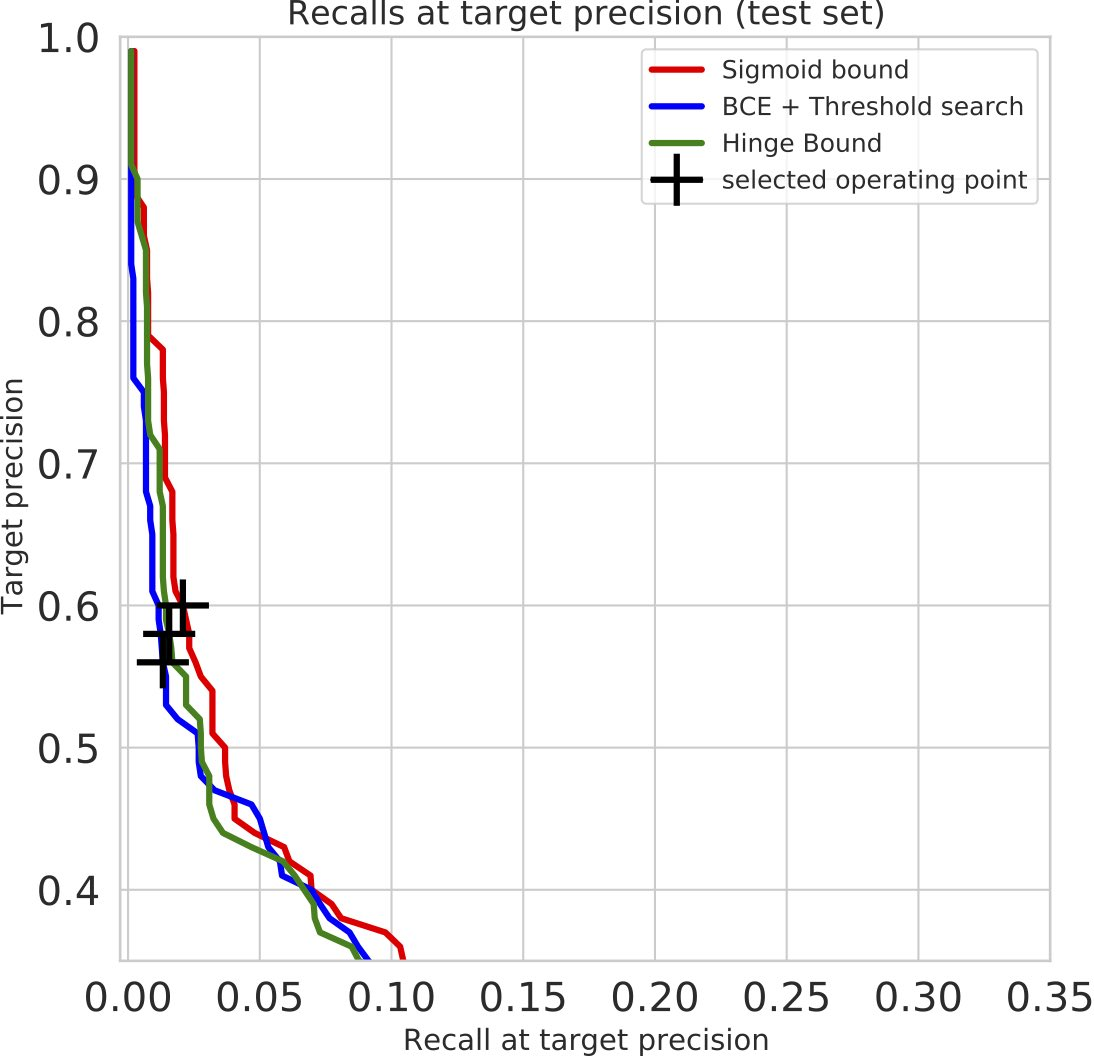
\includegraphics[width=0.9\textwidth]{content/chapters/false_alarm_control/figures/skorch_lr_recalls_at_various_target_precisions_test_EICU.jpg}
    %\includegraphics[width=60mm]{figures/skorch_lr_recalls_at_various_target_precisions.pdf}
    \caption[Improvement in deployment scenario performance for predicting in-hospital mortality (in eICU) with our sigmoid bounds]{Predicting in-hospital mortality on eICU in a deployable scenario (making a prediction every 12 hours), using target precisions of $\alpha=0.7$ on train and $\alpha'=0.6$ on valid. Our proposed sigmoid bound improves precision by 0.02 (100's of fewer false alarms across the 14518 patient-stays in the test set), and improves recall by 0.014 (100's more truly at-risk patients identified).
    % Note that on lower target precisions, the sigmoid bound achieves a poorer recall, because our model is trained with the objective of maximizing recall with a minimum precision of $\alpha=0.7$.
    }%endcaption
    \label{fig:results_per_stay_slice_eicu}
    \vspace{-2.5mm}
\end{figure}